\documentclass[10pt,conference,compsocconf]{IEEEtran}

%\usepackage{times}
%\usepackage{balance}
\usepackage{url}
\usepackage{graphicx}	% For figure environment
\usepackage{subcaption}


\begin{document}
\title{Computational Intelligence Lab Project:\\ Road Segmentation}

\author{
  Igor Pesic\\
  Department of Computer Science,\\ ETH Zurich
  \and
  Felipe Sulser\\
  Department of Computer Science,\\ ETH Zurich
  \and
  Minesh Patel\\
  Department of Computer Science,\\ ETH Zurich
}

\maketitle

\begin{abstract}
  Image segmentation of the aerial road images has become a significant part of the research in the recent years.
  The use cases are numerous and we are going to focus on the simpler, but still very useful part, namely just the road
  segmentation. Our task is to classify the pixels as either road or background. To achieve our goal we have combined
  techniques proposed in several other papers and have adjusted these to suite our requirements and resources best as possible.  
  The main part of our solution is a convolution neural network (CNN). Beside it, we apply the techniques for data augmentation,
  feature selection and post-processing. The results we obtained with our solution are close to the state-of-the-art
  solutions proposed in the other papers, however our model is much simpler.
\end{abstract}

\section{Introduction}

The goal of this work is to segment out the road on the aerial images. The problem is to decide what pixels
represent the road and what pixels are not the road. Even though we would ideally like to have a pixel-wise
granularity, we are proposing an approach that achieves patch-wise granularity which is, in many cases good enough,
especially in this project. This also simplifies the problem substantially since each patch has only value 0 (no road) or 1 (road). \\
\\
For the CNN, we have implemented a novel solution which combines multiple similar other works on this topic 
and also extends it by adding novel ideas. The focus of our work was the design of the
CNN but we also invested a substantial amount of effort into denoising in order
to improve the results obtained by CNN.\\
\\
This report has the following structure: in Section \ref{sec:Data} we explain all the steps we do before training
and evaluating the model, in Section \ref{sec:model_and_methods} we describe our model, both CNN and denoising
that comes after that. Finally in \ref{sec:results} we discuss the results achieved with our model.


\section{Data}
\label{sec:Data}

\subsection{Data Augmentation}
\label{sec:data_aug}
The original data set consisted of 100 labeled aerial images of road maps. As our approach consists of a
deep neural network, we consider that the given data is not enough and thus we try to augment it to expand it further.
For data augmentation, we first rotate all the images by 90 degrees and to mirror them. Beside the obvious increase
in the training data size, this approach also makes our model more robust. Furthermore we have noticed that the 
predictions on the diagonal roads were much worse than on the horizontal and vertical ones. This appears to be due to
the lack of diagonal roads in our original data set. In order to fix this, we pick 9 images with diagonal
roads and highways which we rotate again by 180 and 270 degrees. Finally, we have noticed some inconsistencies
in the labeling of some images  in the dataset and we have decided to discard those from our training data (i.e. a building classified as a road and viceversa). At the end, our data set has 309 images in total, created by rotations and by augmentation of diagonal roads.

\subsection{Feature extraction}
\label{sec:feature}
In the baseline model we split the image in patches of size $16\times16$ pixels. This provided granularity
that was good enough, but it lacked the information about the surroundings. In order to address that, we have come up
with solution that we called \textit{added context}. We have also found that other authors propose a similar approach to enhance the context of a patch such as in Mnih et al. 2010 \cite{Mnih2010} and Alina Elena 2016 \cite{mthesis}. The approach, that enhances the context of a patch, first splist the image in $16\times16$ patches and then adds the 
surroundings area to it so that patches have the total size of $64\times64$ pixels. The difference between patches is
shown in \ref{fig:patches}. Labels are based solely on the original $16\times16$ patch, however in order to classify them correctly, the input is augmented with the context of the small patch.

\begin{figure}
\centering
\begin{subfigure}{.5\columnwidth}
  \centering
  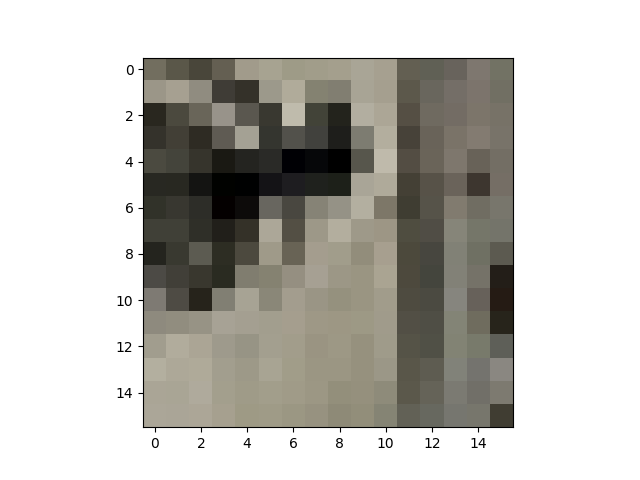
\includegraphics[width=.8\linewidth]{orig_patch.png}
  \caption{Original patch}
\end{subfigure}%
\begin{subfigure}{.5\columnwidth}
  \centering
  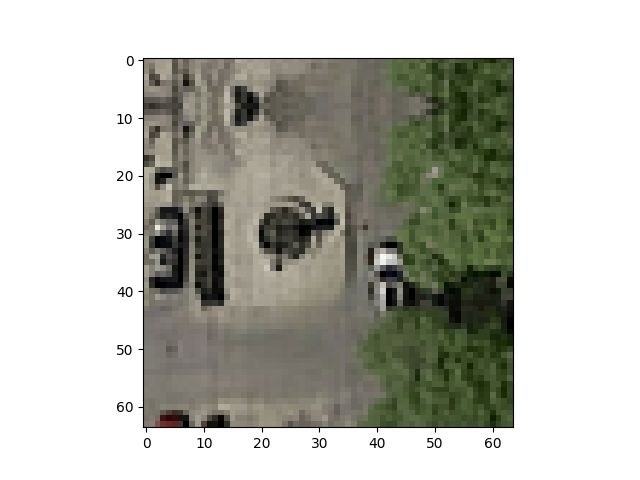
\includegraphics[width=\linewidth]{cont_added_patch.png}
  \caption{Context added patch}
\end{subfigure}
\caption{Context augmentation for patches}
\label{fig:patches}
\end{figure}

We have chosen the patch size empirically by trying out different context-added sizes and 64 turned out to bring the
best score on the Kaggle competition\footnote{\url{inclass.kaggle.com/c/cil-road-segmentation-2017}}.

\subsection{Class balancing}
\label{sec:balance}
Because the dataset was very unbalanced (i.e. the number of background patches was approximately three times bigger than the number of road patches, we had to balance the data so that both classes have a similar number of datapoints. Balancing the data helps reduce the bias towards a certain value in the form of a prior, which is due to the error minimization we are performing. We have done that by 
equalizing the number of patches in both classes, i.e. by randomly picking a limited number of background patches.



\section{Models and Methods}
\label{sec:model_and_methods}
\subsection{Baseline Model}
The baseline model works on batches of $16 \times 16$ patches.\\
 Its configuration is as follows:
 $IN(3, 16\times16)
-C(32, 5\times5 /1) - MP(2 / 2) - C(64, 5\times5 /1) - MP(2 / 2)
-FC(512)-FC(2)$\\
Where:
\begin{itemize}
\item $IN(a,b\times c)$ -- Input image of $a$ channels and size $b \times  c$
\item $CONV(a,b\times c / d)$ -- Convolution layer with depth $a$, window size $b\times c$ and stride $d$
\item $FC(a)$ -- Fully Connected layer of size $a$
\item $MP(a / b)$ -- Max Pooling layer of size $a$ with stride $b$
\end{itemize}

The weights of the network are L2 regularized and the optimizer used is the Momentum Optimizer  with an exponential decaying learning rate with a decay rate of 0.95 and starting at 0.01.
Each convolutional layer is followed by a rectified linear unit ($RELU$) and the activation function in the Fully Connected layers are the identity function .
In the end, the softmax function is applied to the output of the last Fully Connected layer. 
\subsection{Improved CNN Architecture}
The core of our work is the CNN design. We have got the main idea for the architecture
of the network from Alina Elena \cite{mthesis}. In this design, they connect both a VGG network \cite{vgg} and an AlexNet network \cite{alexnet} to create a dual stream network that takes as input the local patch to be predicted and the whole image as context.
Our solution takes this network as inspiration, however it only takes the local information as input. This decision was done due to limited data and also because empirically the results obtained with it were good.

Our CNN network can be described as follows: \\
$IN(3, 64\times64)
-C(64, 3\times3 /2) - MP(2 / 2) - C(128, 3\times3 /2) - MP(2 / 2)
-C(256, 3\times3 /2) - MP(2 / 2) - C(512, 3\times3 /2) - MP(2 / 2)
-FC(2048)-FC(2048)-FC(2)$\\

Additionally all convolutional layers are followed by rectified linear units ($RELU$) layer. The output of the CNN is the softmax function for the two classes and we use the Adam optimizer \cite{adam}.

To reduce overfitting, we initialize the parameters of the network using xavier's initialization algorithm \cite{xavier} and we also use a dropout rate of 0.5 on all the Fully Connected layers during training.
\subsection{Error function}
Our CNN model reduces the log-loss, but for the evaluation we have used two other loss metrics. The first one was
the classification error and it was used on the validation set that helped us find the right number of training epochs. 
Further discussion on that will follow in the next section. The second one was the F-1 score to calculate
the test error. The latter was given by the Kaggle competition.


\subsection{Model hyper-parameters}
Since we used the Adam optimizer, there were not many parameters to tune. One parameter was the batch size, which we 
have not changed from the baseline model since in the one of previous exercises we have learned the it should nether be too
big nor too small, so we found 32 to be a good choice. The only other parameter to tune was the number of training epochs.
This one we have empirically chosen to be (TODO: state the number) based on training the model on 90 images and 
validating it in every epoch on the other 10 images. The Figure (TODO: ref the plot of validation error) shows
how the validation error changes with the number of epochs. Beside these, there were no further hyper-parameters to tune.


\subsection{Post-processing}
In order to improve the output obtained from the CNN network, we perform a post-processing step that helps reduce the noise of the output image and correct some prediction errors. Errors may appear in the image due to the inconsistencies in the roads. As an example, objects that overlap with roads such as cars or trees might have a negative effect on the classification due to their difference in color and shape in contrast with the road. Furthermore, structures like rooftops might sometimes appear like roads.\\
\subsubsection{Model Description}
We propose an approach that first denoises the image and then performs a prediction on the patches. Given the output of the CNN as a grayscale image, we perform a denoising using wavelets. Following the denoising, we convert the image to binary representation (either black or white patches) and then we perform a prediction of the \textit{border patches} using a Multilayer Perceptron (MLP). We tried other models such as SVM (or SVC for classification) and Random Forest, however we obtained the best results with the MLP. Finally, the last step changes a patch's color if at least 7 of a patch's 8 neighbors have a different color, we change it because it is highly likely that it is a misclassified patch if 7 or more of its neighbors have a different color.

In figure \ref{fig:denoising} we can see the outputs of each step. We start with the raw CNN output, we then apply the wavelet denoising, and afterwards we apply the MLP to the border patches only and fill the patch color with the neighbouring technique.
\subsubsection{Wavelet denoising}
For the denoising, we choose wavelets because the results obtained were smooth and appropiate for road images. The wavelets used are Daubechies 1 wavelets. Furthermore the denoising is done assigning the hyperparameter sigma to 3. 
\subsubsection{Multilayer Perceptron classifier}
The input datapoints of the classifier are patches surrounded with context. For the patches, we consider a window of $11\times11$ patches, with the current one to be classified centered. Also, we do not classify all the patches in the image, only the \textit{border patches}. A patch is considered a \textit{border patch} if 5 of its 8 immediate neighbors have a distinct color. We only consider these patches because we observed that the other patches are generally correctly classified as the raw output of the CNN is not so noisy compared to the baseline's output.\\
For the structure of the classifier itself, the parameters were found using a cross validated grid search. The best settings found are to use two hidden layers of size 50 each and to use the logistic activation function. Finally the training of the MLP was done on the 309 groundtruth images that we obtain using data augmentation techniques.

\begin{figure}
\centering
\begin{subfigure}{.3\columnwidth}
  \centering
  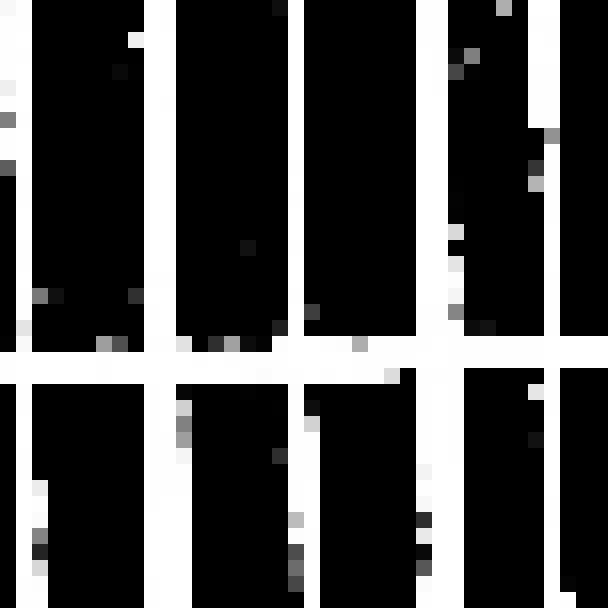
\includegraphics[width=.8\linewidth]{output_cnn_raw.png}
  \caption{Raw CNN output}
\end{subfigure}%
\begin{subfigure}{.3\columnwidth}
  \centering
  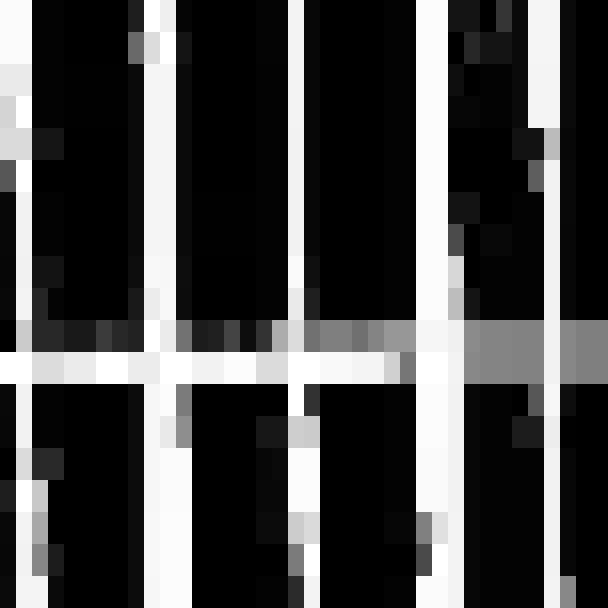
\includegraphics[width=.8\linewidth]{only_wav.png}
  \caption{Wavelet denoising}
\end{subfigure}
\begin{subfigure}{.3\columnwidth}
  \centering
  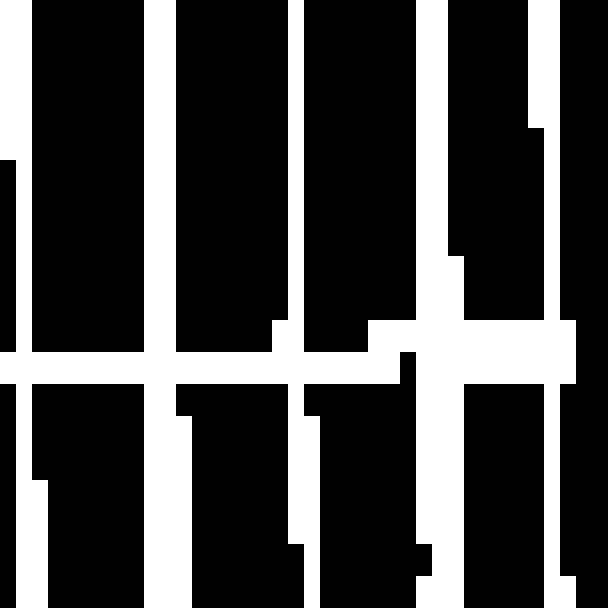
\includegraphics[width=.8\linewidth]{final_res.png}
  \caption{Wavelet + MLP + Neighbor}
\end{subfigure}
\caption{Post-Processing steps}
\label{fig:denoising}
\end{figure}


\section{Results}
\label{sec:results}
\subsection{Implementation}
The model presented here is implemented using tensorflow for the CNN and the denoising was developed using sklearn. The CNN was trained on an Microsoft Azure NV6 instance for 20 hours and 52 minutes using one kernel of the Nvidia Tesla m60 GPU using 2048 CUDA cores provided by the instance. Furthermore the post-processing part was also trained on the Azure instance. The training of the MLP using 6 jobs was done in 2 hours and 51 minutes for the Grid Search method in order to find the optimal parameters.
\subsection{Score}
\subsection{Comparison to baseline model}
The baseline model achieves an F1 score of 0.73723 on the public Kaggle competition, which is significantly lower than the one obtained by our model. Furthemore, the output images obtained by the baseline model are noisy, with patches of roads completely isolated which is something that does not happen on roads.


\section{Conclusions}
\label{sec:conclusions}
In this paper we have discussed a novel method to solve road segmentation on satellite images. The relatively deep CNN presented seems to be a good compromise between ease of train for small dataset and accuracy. Furthermore, post-processing is an important step for road segmentation. The prior knowledge of knowing that we are predicting roads, allows the training of models for image denoising that take into account the overall shape of the roads.\\
Regarding the score, despite the lack of input data it achieves a general high score close to state-of-the-art methods. However this could be improved by making the network more deep and with a further increase in the dataset, something which is left as an idea for further work.




\bibliographystyle{IEEEtran}
\bibliography{howto-paper}
\end{document}